
\chapter{USER RESPONSIBILITIES} \label{chapter:userresponsibilities}

There are a few things that you need to make sure are formatted and/or input correctly for the automation to work correctly.
 This chapter describes some of these things.

\begin{figure}
    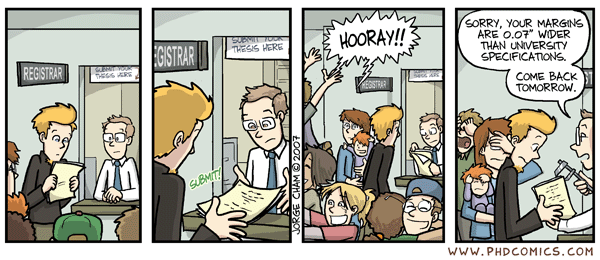
\includegraphics[width=\textwidth]{static/phdcomics}
    \caption[
        The ``short'' caption.
    ]{
        The ``short'' caption.
        Make sure the ``short'' caption and the first sentence of the ``full'' caption are identical.
    }
    \label{fig:phdcomics}
\end{figure}

\section{Front Matter}

Most of the front matter is automatically compiled given the various variable definitions in the preamble of the main tex file.
 You need to fill these out to include your name, degree type, department, etc etc etc.
 If you have a very large number of committee members, or a very long thesis title, or some other special requirement of the front matter, you may need to edit the spacing between individual lines in the class file.

\section{Names of Stuff}

Capitalization and proper punctuation are the responsibility of the user.
 Chapters should be in all caps.
 There is no logic for splitting very long titles across multiple lines, so consider keeping chapter and section titles short enough to fit on a single line.

\subsection{Nomenclature}

There is logic for automatically compiling a \texttt{nomenclature} page.
 If you want something Listed in the Nomenclature (LITN\nomenclature{LITN}{Listed in the Nomenclature}), then use the \texttt{\textbackslash nomenclature} command the first time it appears in your text.
 The auxiliary file for the nomenclature is not automatically generated, and you must manually create it when you require an updated nomenclature page (if you have a nomenclature) with \texttt{makeindex ms.nlo -s nomencl.ist -o ms.nls}.

\subsection{Figures and Tables}

\begin{table}[!t]
  \begin{center}
    \caption{The ``full'' caption.}
    \label{table:theonlytable}
    \begin{tabular}{llll|ll|ll}
        &   & \multicolumn{6}{c}{\textbf{Predicted}} \\
        &   & \multicolumn{2}{c}{\textbf{Method 1}} & \multicolumn{2}{c}{\textbf{Method 2}} & \multicolumn{2}{c}{\textbf{Method 3}} \\
        &   & -    & +    & -    & +    & -    & +    \\
      \multirow{2}{*}{\textbf{True}}
        & - & 14   & 5    & 16   & 3    & 0    & 19   \\
        & + & 14   & 5    & 10   & 9    & 0    & 19
    \end{tabular}
  \end{center}
\end{table}

The table of contents automatically uses the ``short'' caption option for the \texttt{caption} command (or the ``full'' one if the ``short'' one is not defined).
 However, the grad school requires that this matches the first sentence of your ``\emph{full}'' caption.
 You must make sure that the ``short'' and the first sentence of the ``full'' captions agree.

If you have some class of object in your thesis that is like ``figure''s and ``table''s but isn't quite them, the grad school may let you have a separate list in the table of contents for those things.
 For example, in computer science you may have a bunch of ``algorithms'' that you want to make a list of, or in math you may want a list of ``theorems''.
 There is logic in the class file for automatically creating a list of algorithms.
 That logic should be easily repurposed/extended to arbitrary types of things, depending on your field.
 See the \texttt{alg} command in the \texttt{userresponsibilities.tex} file (this file), and also in the class file for a starting point.


\begin{algorithm}[!t] 
    \caption{Localized Classifier Decision Surface Projection}
    \label{algorithm:localsvmscms}
    \alg{Localized Classifier Decision Surface Projection}
\begin{algorithmic}
  \STATE given $A, K, X, q$
  \STATE $y \leftarrow q$
  \REPEAT
    \STATE $f_q \leftarrow A_{K(q,X)}$
    \STATE $y \leftarrow proj(y, DS(f_q))$
  \UNTIL {convergence}
  \RETURN $y, f_q$
\end{algorithmic}
\end{algorithm}

\subsubsection{Subsubsubsubsubsections}

The logic for nested sections is defined down to the \texttt{subsubsection} (3rd level) division.
 If you have \texttt{subsubsubsubsubsection}s in your thesis, consider adding the appropriate spacing logic to the class file.

\section{Citations}
 
Some pointers on the use of et al., as there are options.  You can list all authors (3 or more) for the first citation of the specific authors in your paper and then use the first author’s name, et al., for the subsequent citations for the particular authors.  If there are only two authors, you must list both always. If there are 6 or more authors, you can use et al. for the first and subsequent citations.  If you start your paper using et al. for 3 or more authors, you must do so consistently throughout the paper, regardless of it being the first citation. 

There are several different ways to format your references.  You must follow a specific and acceptable formatting style.  The Graduate School highly recommends using available software to help you keep track of your references.  Most software will export citations into bibtex format as a \texttt{.bib} file.  After properly including your citations \cite{bottou1992local}, the \texttt{bibtex} command will properly arrange all of your citations for inclusion in the references section.
